\documentclass[../main.tex]{subfiles}

\begin{document}
    \chapter{Dialectology}
    \section{Linguistic Studies}
        In dialectology, the main goals of the discipline are:
        \begin{itemize}
            \item to understand how language can vary according to regional and sociological factors,
            \item how can these changes be tracked and interpreted, and
            \item the significance in development of language.
        \end{itemize}

        \exmp{Linguistic Survey of India}{Conducted by Sir George Grierson from 1894--1928. \par
        
        \textbf{Methodology}\par
        Participants were asked to (i) read a standard passage in their language and (ii) translate a few phrases that were used in daily life. \par

        \textbf{Results}\par 
        Grierson found that there were 179 languages and 544 dialects spoken in India. \par

        \textbf{Criticisms} \par
        The participants only involved teachers and officials, and not all areas of India were represented. The workers hired to collect data may not be as sufficiently trained either. Spelling was also an issue as rules were not standardised, a certain pronunciation could have been recorded as different spellings and vice versa.
        }

        \edfn{Isogloss}{An isogloss is a line drawn on a map separating areas according to a particular linguistic feature such as lexis, sounds, grammar. They mark clearly areas which a feature is found from those adjacent areas which it is not recorded or occurs exceptionally.}

        \exmp{Isogloss of France}{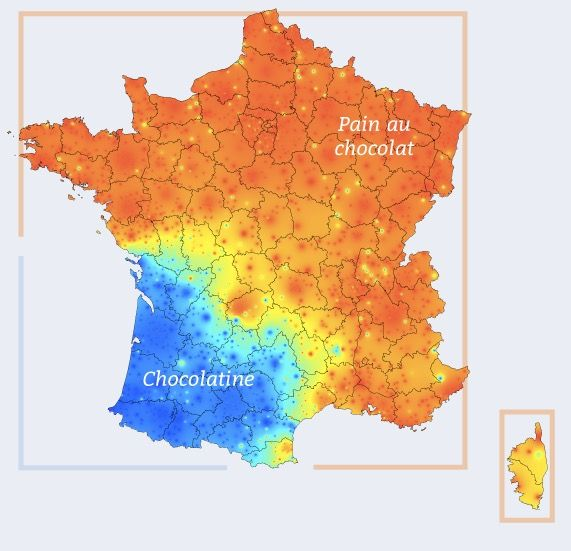
\includegraphics[width=\textwidth]{content/graphics/isogloss.jpg}}

        \section{Dialect Levelling}
        \edfn{Dialect Levelling}{Dialect levelling refers to the means by which dialect differences decrease.}
        Some reasons for dialect levelling are: \begin{itemize}
            \item migration within a country,
            \item lateral (geographical) mobility,
            \item vertical social mobility,
            \item positive approach to new languages,
            \item gender, and
            \item desire for uniqueness.
        \end{itemize}

        \section{Issues with Traditional Dialectology}
        \begin{itemize}
            \item Test items are too narrow and treated as separate entities without context.
            \item Prosodic features were not recorded.
            \item Setting of the study.
            \item Register.
        \end{itemize}
        
        \section{Social Dialectology Today}
        \begin{itemize}
            \item More focused on why different accents and ways of saying things would arise in a same community.
            \item Speech distinctions identified not just based on geography, but on other social markers such as age, education level, gender, etc.
            \item Typical methodology may look like this: \begin{enumerate}
                \item Identify linguistic features in a community.
                \item Select a suitable sample of people and collect data.
                \item Conduct an interview of continuous speech.
                \item Analyse data, noting the frequency of LFs.
                \item Select relevant social units (SES, gender, etc.).
                \item Ascertain significant correlations between social groups and speech choices.
            \end{enumerate}
        \end{itemize}

        \exmp{William Labov in NYC (1966)}{
            Labov conducted a study on rhoticity in NYC, more specifically the post-vocalic /r/. The study was done in three different department stores: Sak's Fifth Avenue, Macy's, and Kleins. \par
            Hypothesis: The speech of people (sales) in the department stores would reflect to a large extent, the norms of their typical customers. \par
            Consistency of data: Labov would ask about an object located on the \textbf{fourth} (/\textipa{f\textopeno \textturnr T}/) floor. \par
            \begin{table}[H]
                \centering
                \begin{tabular}{ccc}
                    SFA & high SES & rhotic \\
                    Macy's & middle SES & rhoticity pronounced \\
                    Klein's & lower SES & non-rhotic
                \end{tabular}
            \end{table}
            In the case of Macy's, it is likely to be a case of hypercorrection.
        }
        
        \edfn{Hypercorrection}{Hypercorrection is a non-standard use of language that results from the over-perception of a perceived rule of language usage prescription.}

        \section{Summary}
        In summary, linguists and dialectologists are alert to nuances in language, such as prosodic features. As we observe these differences, it would also be good for us to think about why these variations exist.

\end{document}
